\documentclass{article}

\usepackage{lipsum}
\usepackage{color}
\usepackage{amsmath}
\usepackage{graphicx}
\usepackage{float}
\usepackage{wrapfig}
\usepackage{epigraph}
\usepackage{csquotes}




% \NewEnviron{First_scientific_papers}{}



\title {CSE300\textunderscore Assignment1\\Introduction to\LaTeX\\Albert Einstein}
\author{Subangkar Karmaker Shanto\\Student ID: 1505015}

\date{}

\begin{document}
\begin{titlepage}
\maketitle
\thispagestyle{empty}
\null
\vfill
\begin{figure}[h]
    \centering
    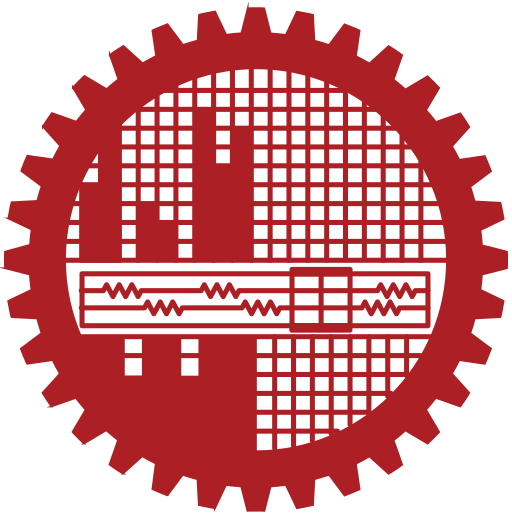
\includegraphics[width=.25\textwidth]{figures/logoBIRN.png}
    \label{fig:logo}
\end{figure}
\begin{center}
Department of Computer Science and Engineering \\Bangladesh University of Engineering and Technology\\(BUET)\\Dhaka 1000 \\
\date{\today}
    
\end{center}
\end{titlepage}

\newpage

\tableofcontents

\newpage


\section{\textcolor{magenta}{Introduction}}

\begin{displayquote}
"Everybody is a genius. But if you judge a fish by its ability to climb a tree, it will live its whole life believing that it is stupid." - {\textit{Albert Einstein}}
\end{displayquote}





\begin{wrapfigure}{r}{0.55\textwidth}
\vspace{-10pt}

\begin{center}
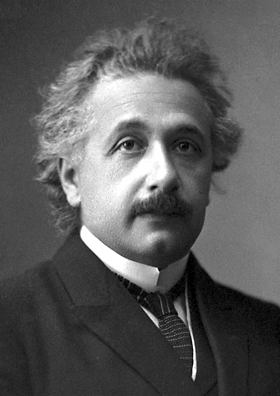
\includegraphics[width=.5\textwidth]{figures/Albert_Einstein_(Nobel).png}
\end{center}

\vspace{-10pt}
\caption{Albert Einstein}
\vspace{-10pt}
\end{wrapfigure}

\textbf{Albert Einstein} (14 March 1879 \– 18 April 1955) was a German-born theoretical physicist who developed the theory of relativity, one of the two pillars of modern physics (alongside quantum mechanics). His work is also known for its influence on the philosophy of science.He is best known by the general public for his mass–energy equivalence formula \textbf{$ E = mc^2 $} (which has been dubbed \textbf{\textit{"the world's most famous equation"}}).He received the \textcolor{red}{\textbf{1921 Nobel Prize in Physics}} \textit{"for his services to theoretical physics, and especially for his discovery of the law of the photoelectric effect"}, a pivotal step in the evolution of quantum theory.


Einstein published more than \textcolor{blue}{300 scientific papers} along with over 150 non-scientific works. His intellectual achievements and originality have made the word "Einstein" synonymous with "genius". Eugene Wigner wrote of Einstein in comparison to his contemporaries that "Einstein's understanding was deeper even than Jansci von Neumann's. His mind was both more penetrating and more original than von Neumann's. And that is a very remarkable statement."



\section{\textcolor{magenta}{Life and career}}
\subsection{Early life and education}
Albert Einstein was born in Ulm, in the Kingdom of Württemberg in the German Empire, on 14 March 1879. His parents were Hermann Einstein, a salesman and engineer, and Pauline Koch. In 1880, the family moved to Munich, where Einstein's father and his uncle Jakob founded Elektrotechnische Fabrik J. Einstein \& Cie, a company that manufactured electrical equipment based on direct current.


The Einsteins were non-observant Ashkenazi Jews and Albert attended a Catholic elementary school in Munich, from the age of 5, for three years. At the age of 8, he was transferred to the Luitpold Gymnasium (now known as the Albert Einstein Gymnasium), where he received advanced primary and secondary school education until he left the German Empire seven years later.


\begin{wrapfigure}{l}{0.45\textwidth}
\vspace{-10pt}

\begin{center}
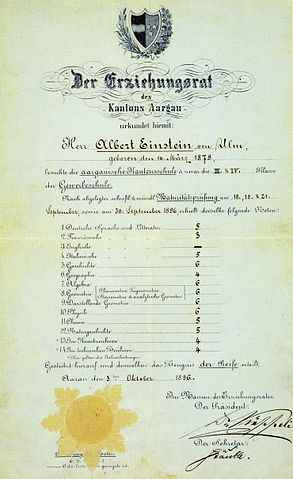
\includegraphics[width=.40\textwidth]{figures/Albert_Einstein's_exam_of_maturity_grades_(color2).jpg}
\end{center}

\vspace{-10pt}
\caption{Einstein's matriculation certificate}
\vspace{-10pt}
\label{fig:matriculation_certificate}
\end{wrapfigure}


Contrary to popular mythology, Einstein always excelled at maths and physics from a young age, reaching a mathematical level years ahead of his peers. The twelve year old Einstein taught himself algebra and Euclidean geometry over a single summer. Einstein also independently discovered his own original proof of the Pythagorean theorem at age 12. A family tutor Max Talmud says that after he had given the 12 year old Einstein a geometry textbook, after a short time "[Einstein] had worked through the whole book. He thereupon devoted himself to higher mathematics... Soon the flight of his mathematical genius was so high I could not follow." His passion for geometry and algebra led the twelve year old to become convinced that nature could be understood as a "mathematical structure". Einstein started teaching himself calculus at 12, and as a 14 year old he says he had "mastered integral and differential calculus".


At age 13, Einstein was introduced to Kant's Critique of Pure Reason, and Kant became his favourite philosopher, his tutor stating: "At the time he was still a child, only thirteen years old, yet Kant's works, incomprehensible to ordinary mortals, seemed to be clear to him."


In 1895, at the age of 16, Einstein took the entrance examinations for the Swiss Federal Polytechnic in Zürich (later the Eidgenössische Technische Hochschule, ETH). He failed to reach the required standard in the general part of the examination,[25] but obtained exceptional grades in physics and mathematics.[26] On the advice of the principal of the Polytechnic, he attended the Argovian cantonal school (gymnasium) in Aarau, Switzerland, in 1895 and 1896 to complete his secondary schooling. While lodging with the family of professor Jost Winteler, he fell in love with Winteler's daughter, Marie. Albert's sister Maja later married Winteler's son Paul. In January 1896, with his father's approval, Einstein renounced his citizenship in the German Kingdom of Württemberg to avoid military service.In September 1896, he passed the Swiss Matura with mostly good grades, including a top grade of 6 in physics and mathematical subjects, on a scale of 1–6. \textcolor{green}{\textit{\textbf{Figure \ref{fig:matriculation_certificate} is that matriculation certificate}}}.


\newpage

\subsection{Academic career}
% \begin{First_scientific_papers}
\subsubsection{First scientific papers}
In 1900, Einstein's paper "Folgerungen aus den Capillaritätserscheinungen" ("Conclusions from the Capillarity Phenomena") was published in the journal Annalen der Physik.On 30 April 1905, Einstein completed his thesis, with Alfred Kleiner, Professor of Experimental Physics, serving as pro-forma advisor. As a result, Einstein was awarded a PhD by the University of Zürich, with his dissertation "A New Determination of Molecular Dimensions".

In that same year, which has been called Einstein's annus mirabilis (miracle year), he published four groundbreaking papers, on the photoelectric effect, Brownian motion, special relativity, and the equivalence of mass and energy, which were to bring him to the notice of the academic world, at the age of 26.
% \end{First_scientific_papers}

\begin{flushleft}
By 1908, he was recognized as a leading scientist and was appointed lecturer at the University of Bern. The following year, after giving a lecture on electrodynamics and the relativity principle at the University of Zürich, Alfred Kleiner recommended him to the faculty for a newly created professorship in theoretical physics. Einstein was appointed associate professor in 1909.

~\newline
Einstein became a full professor at the German Charles-Ferdinand University in Prague in April 1911, accepting Austrian citizenship in the Austro-Hungarian Empire to do so.During his Prague stay, he wrote 11 scientific works, five of them on radiation mathematics and on the quantum theory of solids. In July 1912, he returned to his alma mater in Zürich. From 1912 until 1914, he was professor of theoretical physics at the ETH Zurich, where he taught analytical mechanics and thermodynamics. He also studied continuum mechanics, the molecular theory of heat, and the problem of gravitation, on which he worked with mathematician and friend Marcel Grossmann.
\end{flushleft}




\section{\textcolor{magenta}{Scientific career}}

Throughout his life, Einstein published hundreds of books and articles. He published more than 300 scientific papers and 150 non-scientific ones.On 5 December 2014, universities and archives announced the release of Einstein's papers, comprising more than 30,000 unique documents. Einstein's intellectual achievements and originality have made the word "Einstein" synonymous with "genius". In addition to the work he did by himself he also collaborated with other scientists on additional projects including the Bose–Einstein statistics, the Einstein refrigerator and others.Einstein will never be forgotten for his remarkable contributions in the following fields \& innovations:

\newpage
\begin{enumerate}
    \item Thermodynamic fluctuations and statistical physics
    \item General principles
    \item Theory of relativity and $ E = mc^2 $
    \item Photons and energy quanta
    \item Quantized atomic vibrations
    \item Adiabatic principle and action-angle variables
    \item Wave–particle duality
    \item Theory of critical opalescence
    \item Zero-point energy
    \item General relativity and the equivalence principle
    \item Hole argument and Entwurf theory
    \item Physical cosmology
    \item Modern quantum theory
    \item Bose–Einstein statistics
    \item Energy momentum pseudotensor
    \item Unified field theory
    \item Wormholes
    \item Einstein–Cartan theory
    \item Equations of motion
    \item Other investigations
    \item Collaboration with other scientists
    \item Bohr versus Einstein
    \item Einstein–Podolsky–Rosen paradox
\end{enumerate}



\section{\textcolor{magenta}{Awards and honors}}
Einstein received numerous awards and honors. Some popular of those are followings:

\begin{itemize}
    \item Nobel Prize in Physics, 1921. 
    \item Admission to German Order "Pour La Mérite," 1923. 
    \item Copley Medal, Royal Society of London, 1925. 
    \item Gold Medal, Royal Astronomical Society, London, 1925. 
    \item Max-Planck-Medal, German Physical Society, 1929. 
    \item Benjamin Franklin Medal, Franklin Institute, Philadelphia, 1935
\end{itemize}


\end{document} 